
\documentclass[dvipdfmx,11pt]{beamer}

%全体設定
%\AtBeginDvi{\special{pdf:tounicode 90ms-RKSJ-UCS2}}

\usepackage{bxdpx-beamer}% dvipdfmxなので必要
\usepackage{pxjahyper}
\usepackage{minijs}
\usepackage{otf}
\usepackage{amsmath}
\usepackage{hyperref}
\usepackage[absolute,overlay]{textpos}
\usepackage{comment}
\usepackage{colortbl}
\usepackage{graphicx}

\renewcommand{\kanjifamilydefault}{\gtdefault}
%%\usetheme{Frankfurt}
\usetheme{Warsaw}
\setbeamertemplate{navigation symbols}{} %スライドのボタン?(右下のやつ)を消す
\setbeamersize{text margin left=1.5em,text margin right=1.5em} % 余白なくすやつ

\title{解集合プログラミングを用いた\\配電網問題の解法}
\author{山田 健太郎\\(081631066)}
\date{番原研究室中間発表\\2019年12月20日}
\institute{名古屋大学 工学部\\電気電子情報工学科}

%% テンプレ
\begin{comment}

%%1ページ目
\begin{frame}\frametitle{}
\end{frame}

\end{comment}


%% 本文 %%%%%%%%%%%%%%%%%%%%%%%%%%%%%%%%%%%%%%%%%%%%%%%%%%%%%%%%%%%%%%
\begin{document}

%% タイトル %%%%%%%%%%%%%%%%%%%%%%%%%%%%%%%%%%%%%%%%%%%%%%%%%%%%%%%%%%
\begin{frame}\frametitle{}
  \titlepage
\end{frame}

%%%%%%%%%%%%%%%%%%%%%%%%%%%%%%%%%%%%%%%%%%%%%%%%%%%%%%%%%%%%%%%%%%%%%%
\begin{frame}\frametitle{配電網問題}
 \begin{itemize}
  \item  求解困難な組合せ最適化問題の一種.
  \item  \alert{配電網問題}は,\structure{トポロジ制約}と\structure{電力制約}を満たした上で,
		 損失電力を最小にする
		 スイッチの開閉状態を求める問題である.
  \item  \alert{配電網}とは,\structure{変電所}と\structure{各家庭}との間で構成される
		 電力供給経路のネットワークである.
  \item  配電網の構成技術はスマートグリッドや,災害時の障害箇所の迂回構成などを支える基盤技術として期待されている.
  \item  既存研究
		 \begin{itemize}
		  \item 二分決定グラフを用いた解法[井上ほか '12年]
		  \item[$\Rightarrow$] 実用規模の配電網問題(\structure{\bf スイッチ数468個})の最適解を発見
		 \end{itemize}
 \end{itemize}

\end{frame}

%%%%%%%%%%%%%%%%%%%%%%%%%%%%%%%%%%%%%%%%%%%%%%%%%%%%%%%%%%%%%%%%%%%%%%
\begin{frame}\frametitle{解集合プログラミング(Answer Set Programming; ASP)}
 \begin{itemize}
  \item \structure{ASP言語}は一階論理に基づく知識表現言語の一種である.
  \item \structure{ASPシステム}は論理プログラムから安定モデル意味論[Gelfond and Lifschitz '88]に
		基づく解集合を計算するシステムである.
  \item 近年ではSAT技術を応用した高速ASPシステムが実現され,システム検証,プランニング,
		システム生物学など様々な分野への応用が拡大している.
 \end{itemize}
 \begin{alertblock}{ASPを配電網問題に用いる利点}
   \begin{itemize}
	\item ASP言語の高い表現力を活かし,トポロジ制約を簡潔に記述可能.
	\item 背景理論付きASP技術を用いることにより,電力制約を実装可能.
	\item 充足不能コア等のSAT技術を応用した効率的な最適値探索が可能.
   \end{itemize}
 \end{alertblock}

\end{frame}

%%%%%%%%%%%%%%%%%%%%%%%%%%%%%%%%%%%%%%%%%%%%%%%%%%%%%%%%%%%%%%%%%%%%%%
\begin{frame}\frametitle{研究目的}
 \begin{alertblock}{目的}
  配電網問題に対してASPを適用し,その有効性を評価する.
 \end{alertblock}

 \begin{exampleblock}{研究方針}
  \begin{enumerate}
   \item トポロジ制約のみの配電網問題
   \item 電力制約と目的関数への拡張
  \end{enumerate}
 \end{exampleblock}

 \begin{block}{研究内容}
  \begin{itemize}
   \item トポロジ制約のみの配電網問題に対して,2種類のASP符号化を考案した.
	   \begin{itemize}
		\item 上限,下限に基づく符号化.
		\item ASP言語の表現性を利用した符号化.
	   \end{itemize}
  \item 実用規模の配電網問題,及び,より大規模な問題を用いた評価実験.
	   \begin{itemize}
		\item 問題の規模に関する比較評価.
		\item 生成される制約の数の比較評価.
	   \end{itemize}
  \end{itemize}

 \end{block}

\end{frame}

%%%%%%%%%%%%%%%%%%%%%%%%%%%%%%%%%%%%%%%%%%%%%%%%%%%%%%%%%%%%%%%%%%%%%%
\begin{frame}\frametitle{トポロジ制約のみの配電網問題と根付き全域森}
 \begin{block}{トポロジ制約のみの配電網問題}
  与えられた連結グラフから\alert{変電所を根とする根付き全域森}を見つける部分グラフ探索問題に帰着できる.
 \end{block}

 \begin{exampleblock}{根付き全域森}
  グラフ$G=(V,E)$ ($V$:$G$の頂点集合,$E$:$G$の辺集合)と,
  根と呼ばれる$V$上の頂点$ r_1, \ldots r_k $が与えられたとき,
  $G$上の根付き全域森は以下の条件を満たす$G$の部分グラフ$G'=(V,E'), E' \subseteq E$である.
  \begin{enumerate}
   \item $G'$はサイクルを持たない.
   \item $G'$の各連結成分は,ちょうど1つの根を含む.
  \end{enumerate}
 \end{exampleblock}
\end{frame}

%%%%%%%%%%%%%%%%%%%%%%%%%%%%%%%%%%%%%%%%%%%%%%%%%%%%%%%%%%%%%%%%%%%%%%
\begin{frame}\frametitle{根付き全域森となる配電網の例}

 \begin{figure}[h]
  \centering
  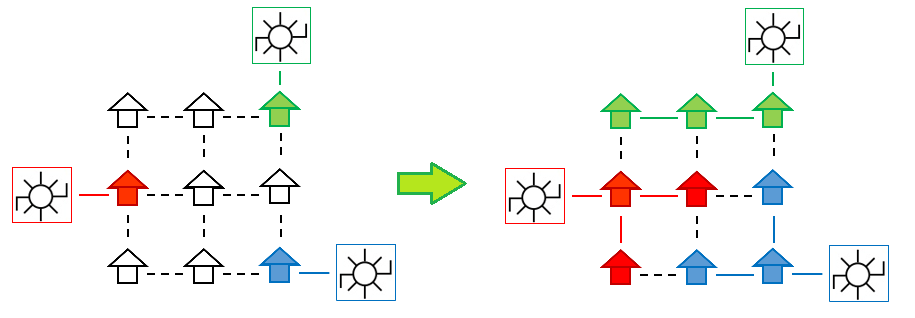
\includegraphics[scale=0.5]{network.png}
 \end{figure}

 \begin{exampleblock}{}
  \begin{itemize}
   \item 供給経路内に閉路が存在しない.
   \item 各家庭は必ず接続され,停電区間が存在しない.
   \item 各家庭はちょうど1つの変電所にのみ接続されている.
  \end{itemize}
 \end{exampleblock}
\end{frame}

%%%%%%%%%%%%%%%%%%%%%%%%%%%%%%%%%%%%%%%%%%%%%%%%%%%%%%%%%%%%%%%%%%%%%%
\begin{frame}\frametitle{提案するASP符号化(1/2)}
 \begin{exampleblock}{符号化の手法}
  \begin{enumerate}
   \item  ある辺$(X,Y)$が,選択され森に含まれることを\structure{$inForest(X,Y)$}と表す.
   \item  頂点$X$について,ある根$R$からその頂点へ到達可能であることを\structure{$reached(X,R)$}とする.
   \item  各根である頂点$R$について\structure{$reached(R,R)$}を生成する.
   \item  頂点$reached(X,R)$とそれを端点にもつ森に含まれる辺$inForest(X,Y)$に対し,
		  もう一方の頂点について\structure{$reached(Y,R)$}を生成し,同じ根から到達可能とする.
   \item  各連結成分が木構造であることから,木の性質より,各連結成分について,
		  選択される\alert{辺の数に関する制約} \structure{頂点の数$- 1$}を導入する.
   \item  各頂点はちょうど1つの根からのみ到達可能であるという,頂点に到達可能な\alert{根の数
		  に関する個数制約}を導入する.
  \end{enumerate}
 \end{exampleblock}
 この個数制約について次の2種類の符号化\structure{dnet1},\structure{dnet2}を考案した.

\end{frame}

%%%%%%%%%%%%%%%%%%%%%%%%%%%%%%%%%%%%%%%%%%%%%%%%%%%%%%%%%%%%%%%%%%%%%%
\begin{frame}\frametitle{提案するASP符号化(2/2)}
 \begin{exampleblock}{}
  \centering
  各頂点は\alert{ちょうど1つ}の根からのみ到達可能である.
 \end{exampleblock}

 \begin{block}{dnet1}
  2つの制約を導入し,それぞれについて生成することにより,ちょうど1つであることを表す.
   \begin{enumerate}
   \item 各根について,\alert{少なくとも1つ}はその頂点に到達可能である.
   \item 各頂点について,\alert{高々1つ}の根から到達可能である.
   \end{enumerate}
 \end{block}

 \begin{block}{dnet2}
  各頂点について,到達可能となる根をを\alert{1つ選択する}という制約を生成する.
 \end{block}

\end{frame}

%%%%%%%%%%%%%%%%%%%%%%%%%%%%%%%%%%%%%%%%%%%%%%%%%%%%%%%%%%%%%%%%%%%%%%
\begin{frame}\frametitle{実験内容}
\renewcommand{\thefootnote}{\fnsymbol{footnote}}
\setcounter{footnote}{1}
2種類のASP符号化 dnet1, dnet2 に対し,以下のベンチマークを行った.

\begin{itemize}
 \item \structure{使用問題:} 全83問
	   \begin{itemize}
		\item 配電網モデル 3問 (スイッチ数: 16個,36個,468個)
		\item \textit{Graph Coloring and its Generalizations}
			  \footnote{https://mat.tepper.cmu.edu/COLOR04/}で公開されている \\
			  グラフ彩色問題のうち,辺の数が10000以下の無向グラフ 80問
			  \footnote{各問題に対し,頂点のうち1/5個をランダムに根として与えた.}
	   \end{itemize}
 \item \structure{ASPシステム:} \textit{clingo-5.4.0}
	   \begin{itemize}
		\item オプション: \textit{trendy}
	   \end{itemize}
 \item \structure{制限時間:} 1800秒/問
\end{itemize}

\end{frame}

%%%%%%%%%%%%%%%%%%%%%%%%%%%%%%%%%%%%%%%%%%%%%%%%%%%%%%%%%%%%%%%%%%%%%%
\begin{frame}\frametitle{実験結果 (1/3)}
% カクタスプロットによる比較
 \begin{figure}[h]
  \centering
  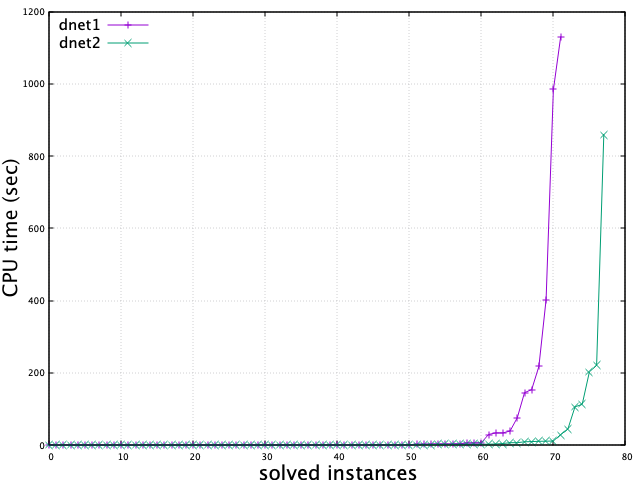
\includegraphics[scale=0.4]{cactus.png}
 \end{figure}

\begin{itemize}
 \item dnet2の方がdnet1よりも制限時間内に解ける問題の数が多い.
 \item 多くの問題においてASPは実行CPU時間が小さい.
\end{itemize}
\end{frame}

%%%%%%%%%%%%%%%%%%%%%%%%%%%%%%%%%%%%%%%%%%%%%%%%%%%%%%%%%%%%%%%%%%%%%%
\begin{frame}\frametitle{実験結果 (2/3)} % 表による比較

\begin{table}[t]
 \centering
 表: 各符号化の問題の規模ごとの解けた問題数\\
 \begin{tabular}[t]{c|c|c|c}
  \noalign{\hrule height 1pt}
  \rowcolor[rgb]{0.46, 0.85, 0.46}
  辺の数 $|E|$ & 問題数 & dnet1 & dnet2 \\
  \noalign{\hrule height 1pt}
  \rowcolor[rgb]{0.94, 1, 0.94}
  $ ~~~~0 \le |E| < ~3000 $ & 46 & 46 & 46 \\
  \hline
  \rowcolor[rgb]{0.94, 1, 0.94}
  $ 3000 \le |E| < ~6000 $ & 22 & 20 & 20 \\
  \hline
  \rowcolor[rgb]{0.94, 1, 0.94}
  $ 6000 \le |E| < 10000 $ & 15 & 6 & \alert{12} \\
  \noalign{\hrule height 1pt}
  \rowcolor[rgb]{0.46, 0.85, 0.46}
  計 & 83 & 72 & \alert{78} \\
  \noalign{\hrule height 1pt}
 \end{tabular}
\end{table}

\begin{itemize}
 \item 比較的小さな規模の問題においては,符号化による性能の違いは \\
	   大きく見られなかった.
 \item 問題の規模が大きな問題に対してはdnet2による符号化はdnet1 \\
	   よりも解ける問題数が多く,より高い拡張性を持つといえる.
\end{itemize}

\end{frame}


%%%%%%%%%%%%%%%%%%%%%%%%%%%%%%%%%%%%%%%%%%%%%%%%%%%%%%%%%%%%%%%%%%%%%%
\begin{frame}\frametitle{実験結果 (3/3)}
% 散布図による比較
 \begin{figure}[h]
  \centering
  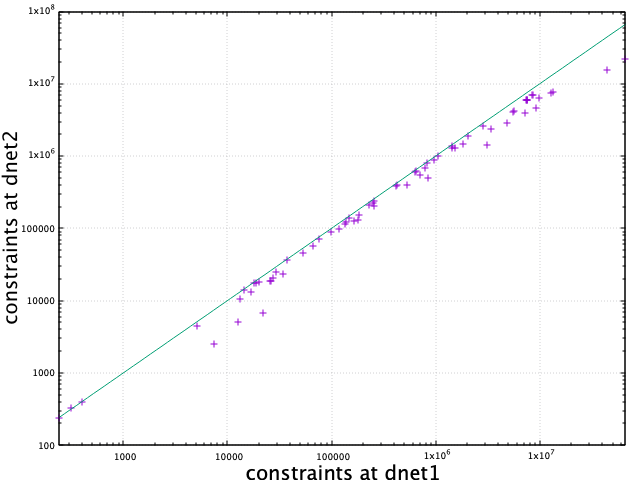
\includegraphics[scale=0.4]{constraints.png}
 \end{figure}

 \begin{itemize}
  \item 全体的にdnet2の方がdnet1による符号化よりも生成される
		制約の数が少なくなっている.
 \end{itemize}
\end{frame}

%%%%%%%%%%%%%%%%%%%%%%%%%%%%%%%%%%%%%%%%%%%%%%%%%%%%%%%%%%%%%%%%%%%%%%
\begin{frame}\frametitle{まとめと今後の課題}
 トポロジ制約のみの配電網問題にASPを適用し,その有効性を評価するために以下を行なった.
\begin{block}{まとめ}
 \begin{itemize}
  \item トポロジ制約のみの配電網問題に対して,2種類のASP符号化を考案した.
		\begin{itemize}
		 \item 考案する符号化をASP言語を用いて,簡潔に記述することができた.
		 \item ASP言語の高い表現力によって,制約の数を減らすことができた.
		\end{itemize}
  \item 実用規模の配電網問題,及び,より大規模な問題を用いた評価実験.
		\begin{itemize}
		 \item 実用規模の配電網問題においては,ASPは高い性能を示した.
		 \item 大規模な問題においても,ASPは問題を解くことができるが,生成される
			   制約の数が少ない方がより高い拡張性を持つと考えられる.
		\end{itemize}
 \end{itemize}
 
 \end{block}

 \begin{exampleblock}{今後の課題}
  \begin{itemize}
   \item さらなる拡張性を持つ符号化の考案.
   \item 根付き全域森の緩和問題,及び,遷移問題への拡張.
   \item 電力制約と目的関数最適化への拡張.
  \end{itemize}
 \end{exampleblock}
\end{frame}
  
\begin{frame}{スマートグリッド}
 \begin{itemize}
  \item \structure{スマートグリッド}とは,電力の供給側,需要側において双方向のやり取りを可能にする
		次世代の\structure{賢い}電力網である.
  \item 従来は一方的に発電所から電力を送り出していたが,通信技術の発達により,使用状況などを
		リアルタイムに把握することが可能となった.
  \item その時に応じた最適な配電網を構成し,制御するといったことが考えられている.
		\begin{itemize}
		 \item 電力需要の変化による,配電ロスの少ない構成.
		 \item 自然エネルギーによる発電量の変動を補う構成.
		\end{itemize}
 \end{itemize}
\end{frame}

\begin{frame}{電力制約}
 \begin{itemize}
  \item 電線の各区間で\alert{許容電流を超えない}.
  \item 電線の抵抗による\alert{電圧降下が許容範囲を超えない}.
		\begin{itemize}
		 \item 遠くに電力を伝えるほど電圧降下が激しくなる.
		 \item 電流が大きいほど電圧降下が激しくなる.
		\end{itemize}
  \item 三相交流抵抗のバランスが必要.
  \item その他にも様々な条件がある.
  \item 電流と電圧が影響し合うのでASP言語だけでは記述できない.
 \end{itemize}
\end{frame}
\end{document}
